\section{General information}
\subsection*{Presentation structure}
\begin{frame}{Structure}
\begin{itemize}
    \item Every section appears in the table of contents and as a navigation title in the upper bar
    \item Every subsection gets shown in the blue box under the main bar
    \item Use a star after (sub)section to not show it in the table of contents
    \item Every slide is represented in its own \textit{frame environment}
\end{itemize}
\end{frame}

\subsection*{Example for tables}
\begin{frame}{Tables}
% To make a table, one uses the tabular environment as in normal \LaTeX
\begin{tabular}{l|l|l|l|l}
 StudentNr & Name & Address & KursNr & KursName \\\hline
 580 & Ola NordmaNN & 5075 Bergen Fv 14 & INF237 & Algorithm Engineering\\
 580 & Ola NordmaNN & 5075 Bergen Fv 14 & INF273 & Meta Heuristics\\
 580 & Ola NordmaNN & 5075 Bergen Fv 14 & INF227 & Logic\\
 256 & Max MustermaNN & 5055 Bergen Lv 85 & INF237 & Algorithm Engineering\\
\end{tabular}
\\[5mm] % distance under the table
To make a table, one uses the tabular environment as in normal \LaTeX\\
You can write normal text before and after the table, remember to use newline
\end{frame}

\begin{frame}{Multiple tables on one slide}
% The answer is hfill and vfill (there might be better ideas)
\begin{tabular}{l|l|l}
 StudentNr & Name & Address\\\hline
 580 & Ola NordmaNN & 5075 Bergen Fv 14\\
 256 & Max MustermaNN & 5055 Bergen Lv 85\\
\end{tabular}
\vfill
\begin{tabular}{l|l}
KursNr & KursName \\\hline
INF237 & Algorithm Engineering\\
INF273 & Meta Heuristikker\\
INF227 & Logikk\\
\end{tabular}
\hfill
\begin{tabular}{l|l}
 StudentNr & KursNr\\\hline
 580 & INF237\\
 580 & INF273\\
 580 & INF227\\
 256 & INF237\\
\end{tabular}
\end{frame}

% after each section, you should give your audience time to think about questions
% you should use some of the duck photos from the images/-folder on these slides to make them happy
\subsection*{Question time}
\begin{frame}{Questions?}
    \begin{figure}
        \centering
        \includegraphics[height = 4.9cm]{images/guillaume9.jpg}
        \caption{Guillaume in front of Tvindefossen}
        \label{fig:guillaume9}
    \end{figure}
\end{frame}

%=================================
\section{Visibility of slides}
\subsection*{Main structure of a frame}
\begin{frame}{A frame}
\begin{itemize}
    \item A frame is not the same as a slide. We can make information appear and disappear on each slides, making up different states of a slide. This is called a frame
    \item The following pages will explain this in detail
\end{itemize}
\end{frame}

\subsection*{Visibility of lists}
\begin{frame}{Itemize: Showing each point after another}
% [<+->] a list shows every point after each other, making n slides of n points
% [<+(2)->] You can adjust the step size
\begin{itemize}[<+->]
    \item Itemize works in the same way as in normal \LaTeX
    \item The command above makes every bullet point appear after each other on n different slides
    \item Everything working like lists has that functionality
\end{itemize}

\end{frame}

% <1-> Defines on which sub-slide something is appearing
\begin{frame}{Itemize: Explicit visibility}
\begin{itemize}
    \item<1-> This information is visible from slide 1 to the end of this frame
    \item<2-> This information is visible from slide 2 to the end of this frame
    \item<2-3> This one will disappear soon
    \item<3-> This one will appear in slide 3
    \item<4-> Did something disappear?
\end{itemize}

\end{frame}

% \pause Pause does exactly the same
\begin{frame}{Itemize: Pause}
\begin{itemize}
    \item Exactly the same can be done using \texttt{pause}
    \item There will be an explicit visibility break before each \texttt{pause} command
    \pause
    \item The next slide will show the rest of the frame or until the next \texttt{pause} is coming
\end{itemize}

\end{frame}

\subsection*{One more pause thing}
% \pause can be used for literally everything on a slide
\begin{frame}{Pause within a text}
Pause can be used within a big text block.\pause~And everything else.\pause~The tilde-symbol is relevant since \LaTeX~would otherwise ignore the space after pause.
\end{frame}

% =====================================
\section{Textblocks}
\subsection*{Textblocks}
\begin{frame}
    \frametitle{Textblocks}
    
    There are three different colours of textblocks in \LaTeX. The colours can be changed, but nobody knows how.
    
    \begin{block}{Remark}
    The names of the environments are \texttt{block}, \texttt{alertblock} and \texttt{examples}
    \end{block}
   
    \begin{alertblock}{Important theorem}
    French is a weird language
    \end{alertblock}
    
    \begin{examples}
    Un bel avion est un avion qui vole bien.
    \end{examples}
\end{frame}

\section{Programme code}
\begin{frame}[fragile]{Example Python}
You can use code on your slides by using the \texttt{minted}, but you need to mark your slides with the parameter \texttt{fragile}
\begin{minted}{python}
for i in range(10):
    print("use Haskell")
\end{minted}
\end{frame}

\begin{frame}[fragile]{Example SQL}
\begin{minted}{sql}
SELECT *
FROM books
WHERE title = "Der satanarchäolügenialkohöllische Wunschpunsch";
\end{minted}
\end{frame}

\section{Other stuff}
% The Visible command tells the frame, which element should be visible on which sub-slide. This works the same as <a-b> for itemize

\subsection*{The visible command}
\begin{frame}{The Visible command}
The \texttt{<a-b>} command from \texttt{itemize} can be used for other slide elements as well. With \texttt{Visible}, you can define a part of the frame only appearing on some sub-slides (from x to y)

\newLine
\visible<2-3>{
 $ G := (V, E)$ with $V$ a set of vertices and $E := \{ (a, b)$ and $(b, a)$ with $a, b \in V $ and $ a \neq b \} $

}
  
\visible<3-3>{
  \newLine
  $ G = (\{1, 2, 3, 4, 5, 6\}, \{(1, 2), (2, 1),
      (1, 3), (3, 1),
      (1, 4), (4, 1), 
      (2, 4), (4, 2), $ \\
  \quad\quad $ (2, 5), (5, 2),
      (2, 6), (6, 2),
      (3, 4), (4, 3),
      (3, 6), (6, 3),
      (5, 6), (6, 5)\}) $
}

\visible<4>{
  \begin{center}
    Lets make that math stuff disappear
  \end{center}
}
\end{frame}


% The "only" command works in the same way as "visible" but hands back space on the slide for other things to show
\subsection*{The only command}
\begin{frame}%{The Only command}
The \texttt{only} command works in the same way as \texttt{visible} but hands back space on the slide for other things to show\\
\begin{center}
  \begin{tabular}{cccccc}
    $ \begin{tabular}{c}1: \\2: \\3: \\4: \\5: \end{tabular} $ &
    $ \begin{bmatrix}-1.28078 \\0.280776 \\-1 \\-1.28078 \\2.28078 \end{bmatrix} $ &
    $\rightarrow$ &
    $ \begin{bmatrix}-1 \\1 \\-1 \\-1 \\1 \end{bmatrix} $ &
    \visible<2>{$\rightarrow$} &
    \visible<2>{\noindent\parbox[c]{2.5cm}{ $V_1 = \{1,3,4\}\\V_2 = \{2,5,6\}$}}
  \end{tabular}\\
  % Note: The math on that slide is no necessarily correct and only has the purpose of representating the use of \LaTeX
  
  \only<1>{ % this graph is visible on slide 1
    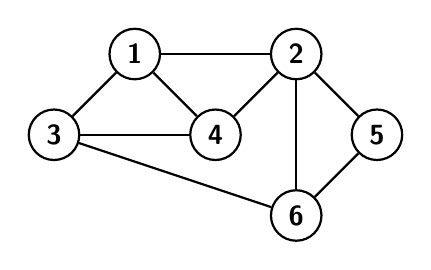
\begin{tikzpicture}[node distance=1.45cm, thick,
                      main node/.style={circle, draw, font=\sffamily\bfseries}]
  
    \node[main node] (1)                    {1};
    \node[main node] (3) [below left  of=1] {3};
    \node[main node] (4) [below right of=1] {4};
    \node[main node] (2) [above right of=4] {2};
    \node[main node] (5) [below right of=2] {5};
    \node[main node] (6) [below left  of=5] {6};

    \path
    (1) edge (2)
    (1) edge (3)
    (1) edge (4)
    (2) edge (4)
    (2) edge (5)
    (2) edge (6)
    (3) edge (4)
    (3) edge (6)
    (5) edge (6);
  \end{tikzpicture}
  }
  \only<2>{ % this graph is visible on slide 2
    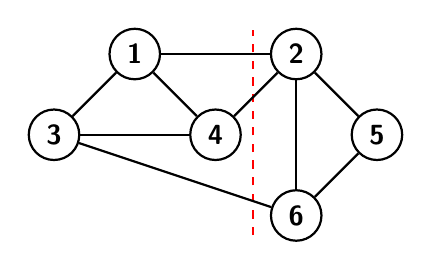
\begin{tikzpicture}[node distance=1.45cm, thick,
                      main node/.style={circle, draw, font=\sffamily\bfseries}]

    \node[main node] (1)                    {1};
    \node[main node] (3) [below left  of=1] {3};
    \node[main node] (4) [below right of=1] {4};
    \node[main node] (2) [above right of=4] {2};
    \node[main node] (5) [below right of=2] {5};
    \node[main node] (6) [below left  of=5] {6};
    \draw[red,thick,dashed] (1.5,-2.3) -- (1.5,0.3);

    \path
    (1) edge (2)
    (1) edge (3)
    (1) edge (4)
    (2) edge (4)
    (2) edge (5)
    (2) edge (6)
    (3) edge (4)
    (3) edge (6)
    (5) edge (6);
  \end{tikzpicture}
  }
\end{center}
\end{frame}

\subsection*{Column layout}
\begin{frame}
    \begin{columns}
    
    \column{0.5\textwidth}
    The representation of a frame in two columns is \textit{of course} possible.
    $$P\stackrel{?}{=} NP$$
    \begin{itemize}
    \item Presentation fanatics can make them appear
    \item after each other
    \item But who would do that?
    \end{itemize}
    
    \pause
    \column{0.5\textwidth}
    To do this, you can use the \texttt{column} command where you define the width of both columns. This frame has a 50:50 proportion.
    \end{columns}

\end{frame}